\documentclass{article}

\usepackage{geometry}
\usepackage{amsmath}
\usepackage{graphicx, eso-pic}
\usepackage{listings}
\usepackage{hyperref}
\usepackage{multicol}
\usepackage{fancyhdr}
\pagestyle{fancy}
\fancyhf{}
\hypersetup{ colorlinks=true, linkcolor=black, filecolor=magenta, urlcolor=cyan}
\geometry{ a4paper, total={170mm,257mm}, top=40mm, right=20mm, bottom=20mm, left=20mm}
\setlength{\parindent}{0pt}
\setlength{\parskip}{0.5em}
\renewcommand{\headrulewidth}{0pt}
\AddToShipoutPictureBG{%
  \AtPageUpperLeft{%
    \raisebox{-\height}{
\includegraphics[width=\paperwidth, height=30mm]{../headerarkav.png}}
  }
}
\rfoot{\thepage}
\lfoot{Competitive Programming - Arkavidia 8.0}
\lstset{
    basicstyle=\ttfamily\small,
    columns=fixed,
    extendedchars=true,
    breaklines=true,
    tabsize=2,
    prebreak=\raisebox{0ex}[0ex][0ex]{\ensuremath{\hookleftarrow}},
    frame=none,
    showtabs=false,
    showspaces=false,
    showstringspaces=false,
    prebreak={},
    keywordstyle=\color[rgb]{0.627,0.126,0.941},
    commentstyle=\color[rgb]{0.133,0.545,0.133},
    stringstyle=\color[rgb]{01,0,0},
    captionpos=t,
    escapeinside={(\%}{\%)}
}

\begin{document}

\begin{center}
    \section*{J. Jelajah Dunia} % ganti judul soal

    \begin{tabular}{ | c c | }
        \hline
        Batas Waktu  & 2s \\    % jangan lupa ganti time limit
        Batas Memori & 256MB \\  % jangan lupa ganti memory limit
        \hline
    \end{tabular}
\end{center}

\subsection*{Deskripsi}
Vidia adalah seorang \textit{reincarnator} yang mampu berpindah tempat dari dunia satu ke dunia lainnya. 

Terdapat $N$ buah dunia di alam semesta. Sebuah dunia dapat direpresentasikan dalam sistem koordinat kartesius dua dimensi. Untuk memisahkan fantasi dengan kenyataan, setiap dunia memiliki sebuah dinding tinggi yang tidak dapat disentuh. Dinding dalam dunia ke-$i$ membentang membentuk garis lurus yang dapat direpresentasikan dalam sebuah fungsi linear $y = x + K_i$. Selain itu, setiap dunia memiliki sebuah portal masuk dan sebuah portal keluar. Pada dunia ke-$i$ portal masuk dan keluar berturut-turut berada pada koordinat $(A_{i}, B_{i})$ dan $(C_{i}, D_{i})$.

Vidia ingin berpetualang menjelajahi setiap dunia. Karena Vidia merupakan seorang \textit{reincarnator}, agar tidak terlalu \textit{overpowered}, di setiap dunia dia dibatasi hanya bisa berjalan dari ($x, y$) ke ($x + 1, y$) atau ($x, y + 1$). Vidia juga tidak boleh menyentuh dinding yang ada di dunia tersebut, artinya Vidia tidak diizinkan untuk menginjakkan kakinya pada koordinat $(p, q)$ yang memenuhi $q = p + K_{i}$.

Sebelum memulai perjalannya, Vidia meminta Anda untuk menemukan banyaknya cara dia dapat berjelajah di setiap dunia dari portal masuk ke portal keluar. Karena jawaban bisa sangat besar, Anda hanya perlu menuliskan jawaban dalam modulo $10^9+7$.

\subsection*{Format Masukan}
Baris pertama terdiri dari satu bilangan bulat positif $N$ ($1 \leq N \leq 2 \times 10^5$), yang menyatakan banyak dunia yang dapat dimasuki Vidia.

$N$ baris berikutnya masing-masing terdiri atas $5$ bilangan, dengan baris ke-$i$ berisi bilangan $K_{i}$ ($-10^6 \leq K_{i} \leq 10^6$), $A_{i}$, $B_{i}$, $C_{i}$, dan $D_{i}$ ($-10^9 \leq A_{i}, B_{i}, C_{i}, D_{i} \leq  10^9$) untuk setiap dunia dari dunia ke-$1$ hingga dunia ke-$N$. Dipastikan untuk setiap dunia, koordinat portal masuk dan keluar memenuhi $0 \leq |A_{i}-C_{i}|+|B_{i}-D_{i}| \leq 10^6$ untuk setiap $i$.

\subsection*{Format Keluaran}
Berisi $N$ baris dengan baris ke-$i$ menyatakan banyaknya cara Vidia berkelana di dunia ke-$i$ setelah di modulo $10^9 + 7$.

\begin{multicols}{2}
\subsection*{Contoh Masukan 1}
\begin{lstlisting}
2
2 -1 3 4 1
1 3 1 6 3
\end{lstlisting}
\columnbreak

\subsection*{Contoh Keluaran 1}
\begin{lstlisting}
0
10
\end{lstlisting}
\vfill
\null
\end{multicols}

\begin{multicols}{2}
\subsection*{Contoh Masukan 2}
\begin{lstlisting}
2
-1 0 2 1 4
-1 1 4 0 2
\end{lstlisting}
\columnbreak

\subsection*{Contoh Keluaran 2}
\begin{lstlisting}
3
0
\end{lstlisting}
\vfill
\null
\end{multicols}

\pagebreak
\subsection*{Penjelasan}
Pada testcase pertama, tidak ada cara bagi Vidia berkelana di dunia ke-$1$.
\begin{figure}[h]
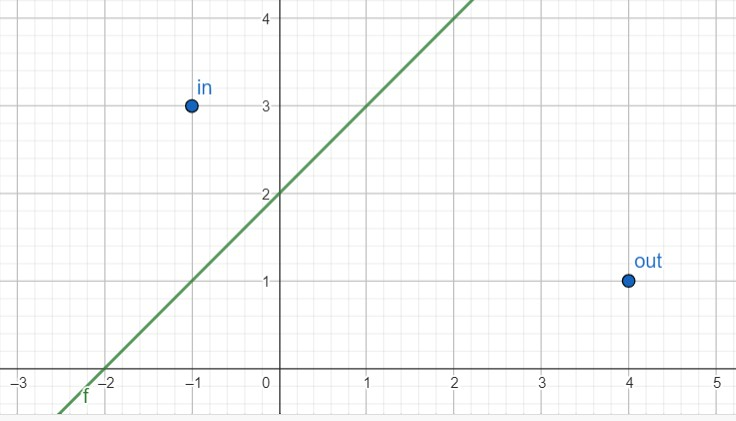
\includegraphics[height=200px]{ilustrasi-1.jpg}
\end{figure}

Sedangkan pada dunia ke-$2$ ada 10 cara bagi Vidia untuk berkelana, salah satunya adalah sebagai berikut: $(3, 1) \xrightarrow{} (3, 2) \xrightarrow{} (3, 3) \xrightarrow{} (4, 3) \xrightarrow{} (5, 3) \xrightarrow{} (6, 3)$ 

\begin{figure}[h]
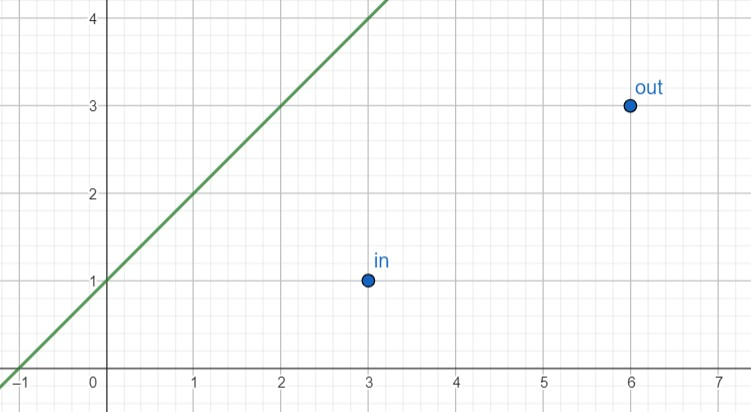
\includegraphics[height=200px]{ilustrasi-2.jpg}
\end{figure}

\end{document}